\chapter{Peluang Bersyarat dan Kebebasan}\label{ch:g12:condprob}

Peluang mengukur ketidakpastian; \omterm{def:g12:condprob:cond}{peluang bersyarat} mengukur bagaimana
keterangan mengubahnya. Mengetahui bahwa \omterm{def:g11:prob:model}{kejadian} $B$ terjadi membentuk ulang
peluang semua \omterm{def:g11:prob:model}{kejadian} lainnya --- suatu mekanisme yang diformalkan Bayes dan
disalahgunakan tiap hari di ruang sidang dan surat kabar. Bab ini menyusun kaidah
pensyaratan dan makna \omterm{def:g12:condprob:indep}{kebebasan} yang tepat.

\section{Ruang peluang (pengingat)}

Percobaan dengan hasil yang berhingga banyaknya dimodelkan oleh \emph{\omterm{def:g11:prob:model}{ruang
sampel}} $\Omega$ (himpunan hasilnya) dan peluang $\P$ yang memberikan kepada
tiap \omterm{def:g11:prob:model}{kejadian} $A \subseteq \Omega$ sebuah bilangan $\P(A) \in \intcc{0}{1}$, yang
aditif atas gabungan yang \omterm{def:g10:proba:operations}{saling lepas} dan dengan $\P(\Omega) = 1$. Ingatlah kaidah dasarnya:
\[
\P(\bar A) = 1 - \P(A),
\qquad
\P(A \cup B) = \P(A) + \P(B) - \P(A \cap B).
\]
Ketika semua hasilnya sama mungkin,
$\P(A) = \frac{\abs A}{\abs\Omega}$ --- dan penghitungan peluangnya menyusut
menjadi teknik pencacahan pada \cref{ch:g12:comb}.

\section{Peluang bersyarat}

\begin{definition}[Peluang bersyarat]\label{def:g12:condprob:cond}
Misalkan $B$ \omterm{def:g11:prob:model}{kejadian} dengan $\P(B) > 0$. Yang disebut \emph{peluang $A$ jika
diketahui $B$}\index{peluang bersyarat} adalah
\[
\pcond{B}{A} = \frac{\P(A \cap B)}{\P(B)} .
\]
\end{definition}

Pemetaan $A \mapsto \pcond BA$ sendiri adalah sebuah peluang (semua kaidahnya
berlaku); pemetaan itu mewakili keadaan pengetahuan yang baru pada orang yang telah
mengetahui bahwa $B$ terjadi.

\begin{proposition}[Kaidah perkalian]\label{prop:g12:condprob:product}
Untuk \omterm{def:g11:prob:model}{kejadian} yang peluangnya tak nol:
\[
\P(A \cap B) = \P(B)\,\pcond{B}{A} = \P(A)\,\pcond{A}{B},
\]
dan secara lebih umum
$\P(A_1 \cap A_2 \cap A_3) = \P(A_1)\,\pcond{A_1}{A_2}\,
\pcond{A_1 \cap A_2}{A_3}$, dan seterusnya.
\end{proposition}

\begin{proof}
Susunlah ulang definisinya; rumus rantainya menyusul lewat pelelaran.
\end{proof}

\begin{theorem}[Hukum peluang total]\label{thm:g12:condprob:total}
\index{hukum peluang total}
Misalkan $B_1, \dots, B_n$ suatu partisi $\Omega$ menjadi \omterm{def:g11:prob:model}{kejadian} yang peluangnya
tak nol. Untuk setiap \omterm{def:g11:prob:model}{kejadian} $A$:
\[
\P(A) = \sum_{i=1}^{n} \P(B_i)\,\pcond{B_i}{A}.
\]
\end{theorem}

\begin{proof}
Himpunan $A \cap B_i$ \omterm{def:g10:proba:operations}{saling lepas} sepasang demi sepasang dengan gabungan $A$, sehingga
$\P(A) = \sum_i \P(A \cap B_i) = \sum_i \P(B_i)\pcond{B_i}{A}$ menurut
kaidah perkaliannya.
\end{proof}

\begin{method}[Pohon peluang]\label{met:g12:condprob:tree}
\omterm{met:g10:proba:tree}{Diagram pohon} menata \omterm{def:g12:condprob:cond}{peluang bersyaratnya}: tiap cabangnya memikul
peluang \omterm{def:g11:prob:model}{kejadian} berikutnya \emph{jika diketahui} lintasan sejauh ini.
\begin{itemize}
  \item Peluang sebuah daun (satu lintasan yang lengkap) adalah \emph{hasil kali}
        peluang di sepanjang cabangnya (kaidah perkalian).
  \item Peluang sebuah \omterm{def:g11:prob:model}{kejadian} adalah \emph{jumlah} peluang
        daun yang mewujudkannya (peluang total).
  \item Peluang pada cabang yang meninggalkan satu simpul berjumlah $1$.
\end{itemize}
\end{method}

\begin{omfigure}
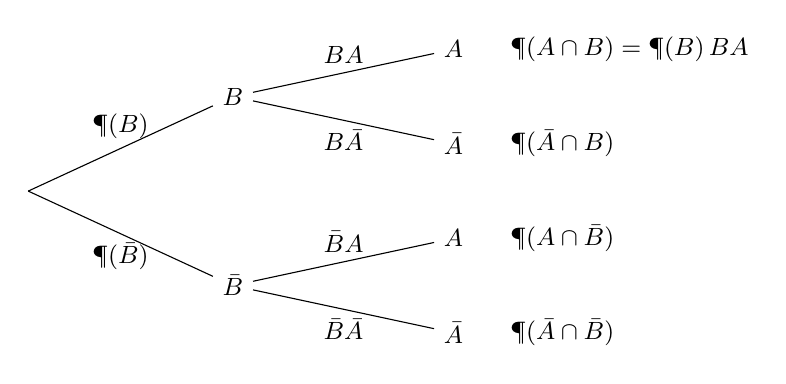
\begin{tikzpicture}[font=\small]
  \coordinate (root) at (0,0);
  \node (B)  at (2.6,1.2)  {$B$};
  \node (Bc) at (2.6,-1.2) {$\bar B$};
  \node (BA)  at (5.4,1.8)  {$A$};
  \node (BAc) at (5.4,0.6)  {$\bar A$};
  \node (BcA)  at (5.4,-0.6) {$A$};
  \node (BcAc) at (5.4,-1.8) {$\bar A$};
  \draw (root) -- (B)  node[midway, above] {$\P(B)$};
  \draw (root) -- (Bc) node[midway, below] {$\P(\bar B)$};
  \draw (B) -- (BA)   node[midway, above] {$\pcond{B}{A}$};
  \draw (B) -- (BAc)  node[midway, below] {$\pcond{B}{\bar A}$};
  \draw (Bc) -- (BcA)  node[midway, above] {$\pcond{\bar B}{A}$};
  \draw (Bc) -- (BcAc) node[midway, below] {$\pcond{\bar B}{\bar A}$};
  \node[anchor=west] at (6.0,1.8)  {$\P(A \cap B) = \P(B)\,\pcond{B}{A}$};
  \node[anchor=west] at (6.0,0.6)  {$\P(\bar A \cap B)$};
  \node[anchor=west] at (6.0,-0.6) {$\P(A \cap \bar B)$};
  \node[anchor=west] at (6.0,-1.8) {$\P(\bar A \cap \bar B)$};
\end{tikzpicture}

{\small \omterm{met:g10:proba:tree}{Pohon} dua tingkat: kalikan sepanjang lintasannya, jumlahkan atas daunnya.
Misalnya $\P(A)$ adalah jumlah peluang daun pertama dan daun
ketiganya.}
\end{omfigure}

\begin{theorem}[Rumus Bayes]\label{thm:g12:condprob:bayes}
\index{rumus Bayes}
Misalkan $B_1, \dots, B_n$ suatu partisi $\Omega$ seperti di atas dan $A$ \omterm{def:g11:prob:model}{kejadian}
dengan $\P(A) > 0$. Maka
\[
\pcond{A}{B_j} =
\frac{\P(B_j)\,\pcond{B_j}{A}}{\sum_{i=1}^{n} \P(B_i)\,\pcond{B_i}{A}} .
\]
\end{theorem}

\begin{proof}
$\pcond{A}{B_j} = \frac{\P(A \cap B_j)}{\P(A)}$; jabarkan pembilangnya lewat
kaidah perkalian dan penyebutnya lewat peluang total.
\end{proof}

\begin{example}[Uji penapisan]\label{ex:g12:condprob:test}
Suatu penyakit menyerang $1\%$ penduduk. Sebuah uji mendeteksinya dengan peluang
$0.99$ (kepekaannya) dan memberi positif palsu dengan peluang $0.05$.
Jika ujinya positif, peluang benar-benar mengidap penyakit itu adalah
\[
\frac{0.01 \times 0.99}{0.01\times0.99 + 0.99\times0.05}
= \frac{0.0099}{0.0099 + 0.0495} = \frac{1}{6} \approx 0.17 .
\]
Walaupun ujinya jitu, lima dari enam positifnya palsu --- sebab
penyakitnya jarang. Mengacaukan $\pcond{A}{B}$ dengan $\pcond{B}{A}$ adalah
\emph{sesat pikir jaksa}.
\end{example}

\begin{omfigure}
\begin{tikzpicture}[font=\small]
  \coordinate (root) at (0,0);
  \node (D)  at (2.6,1.2)  {$D$};
  \node (Dc) at (2.6,-1.2) {$\bar D$};
  \node (DT)  at (5.2,1.8)  {$T$};
  \node (DTc) at (5.2,0.6)  {$\bar T$};
  \node (DcT)  at (5.2,-0.6) {$T$};
  \node (DcTc) at (5.2,-1.8) {$\bar T$};
  \draw (root) -- (D)  node[midway, above] {$0.01$};
  \draw (root) -- (Dc) node[midway, below] {$0.99$};
  \draw (D) -- (DT)   node[midway, above] {$0.99$};
  \draw (D) -- (DTc)  node[midway, below] {$0.01$};
  \draw (Dc) -- (DcT)  node[midway, above] {$0.05$};
  \draw (Dc) -- (DcTc) node[midway, below] {$0.95$};
  \node[omThm, anchor=west] at (5.8,1.8)  {$0.0099$ \ (positif benar)};
  \node[anchor=west] at (5.8,0.6)  {$0.0001$};
  \node[omThm, anchor=west] at (5.8,-0.6) {$0.0495$ \ (positif palsu)};
  \node[anchor=west] at (5.8,-1.8) {$0.9405$};
\end{tikzpicture}

{\small Uji penapisannya sebagai \omterm{met:g10:proba:tree}{pohon} ($D$: mengidap, $T$: uji
positif). Kedua daun positifnya (merah) berbobot total $0.0594$, dan
positif palsunya menyumbang lima perenamnya.}
\end{omfigure}

\section{Kebebasan}

\begin{definition}[Kejadian saling bebas]\label{def:g12:condprob:indep}
Dua \omterm{def:g11:prob:model}{kejadian} $A$ dan $B$ disebut \emph{saling bebas}\index{kebebasan} jika
\[
\P(A \cap B) = \P(A)\,\P(B) .
\]
Ketika $\P(B) > 0$, ini setara dengan $\pcond{B}{A} = \P(A)$: jadi mengetahui $B$
tidak mengubah peluang $A$.
\end{definition}

\begin{proposition}\label{prop:g12:condprob:indepcompl}
Jika $A$ dan $B$ \omterm{def:g12:condprob:indep}{saling bebas}, maka begitu pula $A$ dan $\bar B$ (juga $\bar A$ dan
$\bar B$).
\end{proposition}

\begin{proof}
$\P(A \cap \bar B) = \P(A) - \P(A \cap B) = \P(A) - \P(A)\P(B)
= \P(A)\bigl(1 - \P(B)\bigr) = \P(A)\,\P(\bar B)$.
\end{proof}

\begin{remark}
Janganlah mengacaukan \emph{\omterm{def:g12:condprob:indep}{saling bebas}} ($\P(A\cap B) = \P(A)\P(B)$) dengan
\emph{\omterm{def:g10:proba:operations}{saling lepas}} ($A \cap B = \varnothing$). Dua \omterm{def:g11:prob:model}{kejadian} \omterm{def:g10:proba:operations}{saling lepas} yang
peluangnya tak nol tak pernah \omterm{def:g12:condprob:indep}{saling bebas}: mengetahui yang satu terjadi menjamin
yang lain tidak.
\end{remark}

\begin{definition}[Pengulangan yang saling bebas]\label{def:g12:condprob:repet}
Ketika sebuah percobaan diulang $n$ kali sedemikian sehingga hasil tiap ulangannya
tidak memengaruhi ulangan lainnya, peluang suatu \omterm{def:g12:seq:sequence}{barisan} hasil tertentu
adalah hasil kali peluang masing-masingnya. Inilah model
yang mendasari \omterm{def:g11:prob:rv}{distribusi} binomial (\cref{ch:g12:randvar}).
\end{definition}

\section{Latihan}

\begin{exercise}[$\star$]\label{exo:g12:condprob:1}
Sebuah kartu diambil dari satu pak baku berisi 52 kartu. Hitunglah peluang bahwa
kartu itu raja, jika diketahui kartu itu bergambar (jack, ratu atau raja). Apakah
\omterm{def:g11:prob:model}{kejadian} ``raja'' dan ``hati'' \omterm{def:g12:condprob:indep}{saling bebas}?
\end{exercise}

\begin{exercise}[$\star$]\label{exo:g12:condprob:2}
Sebuah guci memuat 5 bola merah dan 3 bola biru. Dua bola diambil berturut-turut
\emph{tanpa} pengembalian.
\begin{enumerate}
  \item Lukiskan \omterm{met:g10:proba:tree}{pohon} peluangnya.
  \item Hitunglah peluang bahwa keduanya merah, dan peluang bahwa
        bola keduanya merah.
\end{enumerate}
\end{exercise}

\begin{exercise}[$\star$]\label{exo:g12:condprob:3}
Dua dadu setimbang dilempar. Misalkan $A$ = ``jumlahnya $7$'', $B$ = ``dadu
pertama menunjukkan $3$'', $C$ = ``jumlahnya $6$''. Tentukan apakah $A$ dan $B$
\omterm{def:g12:condprob:indep}{saling bebas}, lalu apakah $B$ dan $C$ \omterm{def:g12:condprob:indep}{saling bebas}.
\end{exercise}

\begin{exercise}[$\star\star$]\label{exo:g12:condprob:4}
Sebuah pabrik mempunyai tiga mesin yang berturut-turut menghasilkan $50\%$, $30\%$ dan
$20\%$ keluaran totalnya, dengan laju cacat $1\%$, $2\%$ dan $4\%$.
\begin{enumerate}
  \item Berapa bagian produksinya yang cacat?
  \item Sebuah barang yang dipilih acak ternyata cacat. Berapa peluang barang itu
        berasal dari mesin ketiga?
\end{enumerate}
\end{exercise}

\begin{exercise}[$\star\star$]\label{exo:g12:condprob:5}
Pada \cref{ex:g12:condprob:test}, pada kelaziman penyakit $p$ yang mana (alih-alih
$1\%$) uji positif akan berarti sekurang-kurangnya $90\%$ kemungkinan mengidap? Selesaikan
pertidaksamaannya lalu berilah tanggapan.
\end{exercise}

\begin{exercise}[$\star\star$]\label{exo:g12:condprob:6}
Sekeping uang logam yang berat sebelah jatuh pada sisi gambar dengan peluang $p \in \intoo{0}{1}$.
Uang itu dilempar tiga kali, dan lemparannya \omterm{def:g12:condprob:indep}{saling bebas}.
\begin{enumerate}
  \item Hitunglah peluang \omterm{def:g11:prob:model}{kejadian} $E$ = ``tepat dua gambar''.
  \item Untuk $p$ yang mana $\P(E)$ maksimal?
\end{enumerate}
\end{exercise}

\begin{exercise}[$\star\star\star$]\label{exo:g12:condprob:7}
\emph{(Monty Hall.)} Sebuah hadiah bersembunyi di balik satu dari tiga pintu. Kamu memilih
satu pintu; pembawa acaranya, yang tahu di mana hadiahnya, membuka satu dari dua
pintu sisanya, dan selalu menyingkapkan pintu yang kosong (dengan memilih secara acak jika
keduanya kosong), lalu menawarkanmu untuk berpindah ke pintu tertutup yang lain. Dengan
rumus Bayes, hitunglah peluang menang jika kamu berpindah, dan jika
kamu tidak berpindah.
\end{exercise}

\begin{exercise}[$\star\star\star$]\label{exo:g12:condprob:8}
Sebuah saluran keterangan mengirimkan bit. Tiap bitnya terbalik oleh derau dengan
peluang $\varepsilon = 0.1$, secara \omterm{def:g12:condprob:indep}{saling bebas}. Untuk melindungi satu bit, bit itu dikirim
tiga kali lalu diterjemahkan menurut suara terbanyak.
\begin{enumerate}
  \item Hitunglah peluang bahwa bit yang diterjemahkan itu keliru.
  \item Kata yang diterima adalah $101$. Berapa peluang bahwa bit yang
        dikirim adalah $1$? (Anggaplah $0$ dan $1$ dikirim dengan peluang yang sama.)
\end{enumerate}
\end{exercise}

\section{Soal: Dokter, hakim dan penyaring surat sampah}

\begin{problem}[{Soal akhir pekan --- rumus Bayes melawan
sesat pikir laju dasar: mengapa uji $99\,\%$ dapat berarti $2\,\%$, mengapa
kecocokan satu berbanding sejuta tidak memvonis siapa pun, dan bagaimana kotak suratmu
berpikir}]
\label{pb:g12:condprob:1}
Sebuah uji yang menangkap $99\,\%$ kasusnya kembali dengan hasil positif ---
padahal peluang sesungguhnya mengidap penyakit itu di bawah $2\,\%$. Sebuah profil
DNA yang cocok dengan satu orang di antara sejuta ditemukan --- padahal
tersangkanya besar kemungkinan tak bersalah. Kedua pernyataan itu benar, keduanya
pernah disalahnilai oleh dokter dan pengadilan, dan keduanya diputuskan
oleh satu baris bab ini: rumus Bayes
(\cref{thm:g12:condprob:bayes}). Soal ini melatihnya pada guci,
lalu di klinik, ruang sidang dan kotak masuk.

\medskip
\noindent\textbf{Bagian I --- Kelancaran.}
\begin{enumerate}
  \item Sekeping uang logam yang setimbang memilih guci I ($2$ merah, $1$ biru) atau guci II
        ($1$ merah, $3$ biru), lalu satu bola diambil. Hitunglah
        $\P(\text{merah})$ dengan hukum peluang total
        (\cref{thm:g12:condprob:total}).
  \item Bolanya merah: hitunglah $\P(\text{guci I} \mid
        \text{merah})$.
  \item Satu lemparan dadu: apakah \omterm{def:g11:prob:model}{kejadian} ``genap'' dan
        ``$\leq 4$'' \omterm{def:g12:condprob:indep}{saling bebas}
        (\cref{def:g12:condprob:indep})? Lalu ``genap'' dan
        ``$\leq 3$''?
  \item Dua alarm asap yang \omterm{def:g12:condprob:indep}{saling bebas} masing-masing berbunyi dengan
        peluang $0.9$ ketika ada kebakaran. Dengan memakai
        \cref{prop:g12:condprob:indepcompl}, hitunglah
        peluang bahwa sekurang-kurangnya satu berbunyi.
  \item Dua kartu tanpa pengembalian: hitunglah
        $\P(\text{dua raja})$ dengan kaidah perkalian
        (\cref{prop:g12:condprob:product}).
\end{enumerate}

\medskip
\noindent\textbf{Bagian II --- Sang dokter.}
Sebuah penyakit menyerang $1$ orang dari $1\,000$. Ujinya mendeteksi
$99\,\%$ orang sakit (kepekaannya) tetapi juga berbunyi pada $5\,\%$
orang sehat (positif palsu).
\begin{enumerate}[resume]
  \item Frekuensi alaminya: bayangkan $100\,000$ orang. Berapa
        yang sakit, berapa yang sehat? Berapa positif
        yang dihasilkan tiap kelompoknya, dan berapa positif
        seluruhnya?
  \item Dari cacahnya, hitunglah
        $\P(\text{sakit} \mid \text{positif})$. Resapilah
        kejutannya.
  \item Hitunglah ulang dengan rumus Bayes lalu periksalah
        kecocokannya.
  \item Pada survei, kebanyakan dokter menjawab ``kira-kira
        $99\,\%$''. Sebutkan kedua \omterm{def:g12:condprob:cond}{peluang bersyarat}
        yang diacaukan, lalu jelaskan mengapa laju dasar yang mungil
        itu menggerakkan jawaban yang benar.
  \item Uji kedua yang \omterm{def:g12:condprob:indep}{saling bebas} juga kembali positif.
        Perbaruilah: dengan mengambil $1.9\,\%$ sebagai peluang awal yang baru, hitunglah
        $\P(\text{sakit} \mid \text{dua positif})$. Apa yang sedang dilakukan
        \emph{penimbunan} bukti itu?
  \item Hitunglah $\P(\text{sakit} \mid \text{positif})$ jika
        uji yang sama hanya dipakai pada kelompok berisiko tinggi dengan
        kelaziman $5\,\%$. Simpulkan pelajaran kesehatan masyarakat
        tentang penapisan massal bagi penyakit yang langka.
\end{enumerate}

\medskip
\noindent\textbf{Bagian III --- Sang hakim.}
\begin{enumerate}[resume]
  \item Sebuah profil DNA di tempat \omterm{def:g11:prob:model}{kejadian} cocok dengan satu orang dari
        sejuta. Tersangkanya, yang ditemukan lewat penelusuran pangkalan data
        berisi $10$ juta penduduk kota itu, cocok. Berapa harapan
        banyaknya kecocokan yang tak bersalah di kota itu? Jika hanya diketahui
        kecocokannya, kira-kira berapa $\P(\text{tak bersalah} \mid
        \text{cocok})$?
  \item Sebutkan sesat pikirnya --- peluang mana yang dikutip
        sang jaksa, dan peluang mana yang diperlukan pengadilan? ---
        beserta kesejajarannya yang persis dengan pertanyaan 9.
  \item Jebakan \omterm{def:g12:condprob:indep}{kebebasannya}: dua musibah langka dalam satu keluarga
        pernah dikuadratkan menjadi ``satu berbanding $73$ juta'' dengan
        memperlakukannya sebagai \omterm{def:g12:condprob:indep}{saling bebas}, sehingga memvonis seorang ibu
        yang tak bersalah (perkara Sally Clark). Jika kedua \omterm{def:g11:prob:model}{kejadiannya} berbagi
        faktor risiko keluarga sehingga \omterm{def:g11:prob:model}{kejadian} kedua, jika diketahui yang
        pertama, $5$ kali lebih mungkin daripada laju dasarnya,
        hitunglah ulang orde besarnya --- lalu nyatakan
        pelajarannya tentang mengalikan peluang.
  \item Pihak pembela pun dapat berbuat curang: ``sepuluh orang tak bersalah cocok, jadi
        kecocokannya tidak membuktikan apa-apa'' mengabaikan segala hal lainnya.
        Apa yang dilakukan rumus Bayes dengan \emph{beberapa} keping
        bukti, dan satu kalimat apa yang harus diketahui setiap
        anggota juri?
\end{enumerate}

\medskip
\noindent\textbf{Bagian IV --- Penyaring surat sampah.}
\begin{enumerate}[resume]
  \item Suratmu $40\,\%$ berupa sampah. Kata ``undian''
        muncul pada $15\,\%$ surat sampah dan $0.5\,\%$ surat
        yang jujur. Sebuah pesan memuatnya: hitunglah
        $\P(\text{sampah} \mid \text{undian})$.
  \item Pengulangan yang memperbaiki galat
        (\cref{exo:g12:condprob:8} dilanjutkan): dengan peluang
        terbalik $\varepsilon = 0.1$, penerjemahan menurut suara terbanyak atas
        \emph{lima} salinan gagal dengan peluang berapa?
        Bandingkan dengan sandi tiga salinannya.
  \item Sebuah bit melewati $4$ penerus berderau yang \omterm{def:g12:condprob:indep}{saling bebas}, dan masing-masing
        membalikkannya dengan peluang $0.1$: bit itu tiba dengan benar
        tepat ketika banyaknya pembalikan genap. Hitunglah peluang itu
        dua kali: lewat penjumlahan suku binomialnya, dan
        lewat rumus yang elok,
        $\frac{1 + (1 - 2\varepsilon)^4}{2}$.
  \item Penyaring surat sampah yang sungguhan mengalikan bukti dari banyak kata
        seolah-olah \omterm{def:g12:condprob:indep}{saling bebas} (Bayes yang ``naif''). Mengapa anggapan
        itu salah bagi kata seperti ``menang'' dan
        ``undian'' --- dan mengapa penyaringnya toh bekerja dengan
        baik? (Satu atau dua kalimat.)
  \item Penutup --- Bayes sebagai aritmetika keyakinan: peluang awal
        $\times$ kebolehjadian, normalkan ulang, peluang akhir. Ulangilah
        ketiga vonisnya (klinik, ruang sidang, dan kotak masuk) masing-masing dalam satu
        kalimat, lalu daftarkan ketiga jebakan yang disingkap soal ini:
        laju dasar yang terlupakan, \omterm{def:g12:condprob:indep}{kebebasan} yang palsu, dan
        bukti yang dibaca sekeping demi sekeping.

\end{enumerate}
\end{problem}
